%% Exercice 3

%\ExoSpecs{\TTBF{CalculTVA.sh}}{\TTBF{\RenduDir/src/exo1/}}{750}{640}{\TTBF{write}}
\ExoSpecsCustom{\TTBF{stack\_linked.c}}{\TTBF{\RenduDir/src/}}{750}{640}{Fonctions autorisées}{\TTBF{malloc(3)}, \TTBF{free(3)}, \TTBF{printf(3)}}

\vspace*{0.7cm}

\noindent \ExoObjectif{Le but de l'exercice est d'implémenter une des structures de base : les piles à base de listes chaînées.}

\bigskip

%\noindent Les fonctions demandées dans cet exercice devront se trouver dans une bibliothèque nommée \TTBF{libmystack}.
%Après un appel à la commande \texttt{make} à la racine du projet, il faut que votre chaîne de compilation produise à la racine de votre projet une version statique de la bibliothèque (qui se nommera \TTBF{libmystack.a}) ainsi qu'une version dynamique de la bibliothèque (qui se nommera \TTBF{libmystack.so}).
%
%\bigskip

\noindent Vous devez écrire plusieurs fonctions permettant de gérer des piles à base de listes chaînées, c'est-à-dire des piles exploitant des listes à base de pointeurs.
Un fichier \TTBF{stack\_linked.h} contenant toutes les fonctions exportables à implémenter vous est fourni en annexe.
Vous devrez réutiliser la structure \TTBF{list\_linked} telle quelle issue du fichier \TTBF{list\_linked.h} : \textbf{vous ne devez pas créer de nouvelle structure}.
La liste chaînée ainsi représentée contient deux champs exactement : \textit{elt} (l'élément inséré) et \textit{next} (pointeur vers le maillon suivant de la chaîne).

\smallskip

%\noindent Conceptuellement, les fonctions manipulant des piles de type \TTBF{stack\_ll*} devront pouvoir gérer ces 3 cas :

%\bigskip

%\begin{center}
%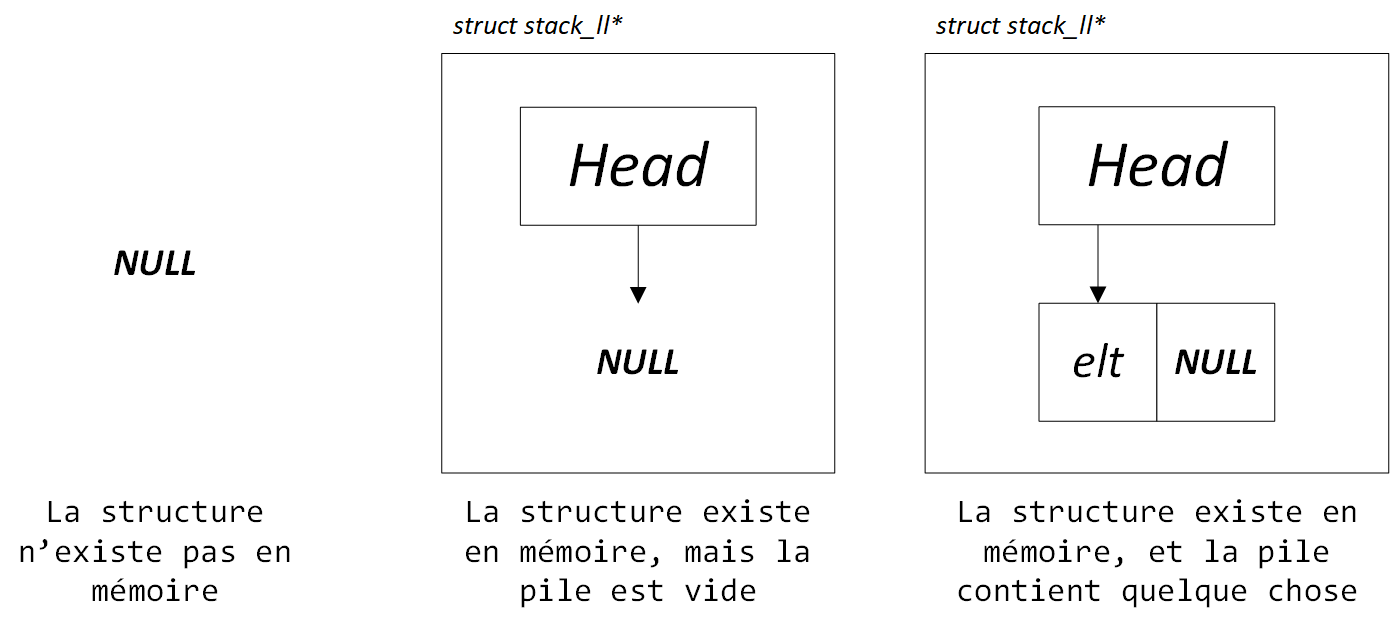
\includegraphics[scale=0.85]{Cours/Piles_Implementation_LL.png}
%\end{center}

\bigskip
%\newpage

\noindent Vous devez implémenter les fonctions suivantes :

\bigskip
%\medskip

\lstset{language=C}
%\begin{lstlisting}[frame=single,title={Liste des fonctions pour une pile avec liste chaînée}]
\begin{lstlisting}[frame=single]
list_linked *push_stack_linked(list_linked *list,
                               int elt);
list_linked *pop_stack_linked(list_linked *list);

int length_stack_linked(list_linked *list);
int is_empty_stack_linked(list_linked *list);

void print_stack_linked(list_linked *list);

int get_head_stack_linked(list_linked *list);

int clear_stack_linked(list_linked *list);
\end{lstlisting}


\clearpage


\subsubsection*{\TTBF{list\_linked *push\_stack\_linked(list\_linked *list, int elt)}}

\noindent Cette fonction empile un nouvel élément, c'est-à-dire qu'elle ajoute un élément en tête de la pile, c'est-à-dire qu'elle ajoute un élément en première position de la liste chaînée donnée en paramètre.

\smallskip

\noindent Si la pile est vide, il faut y créer un premier élément.

\noindent Si l'élément \textit{elt} donné en paramètre est inférieur à $ 1 $, la fonction doit renvoyer un pointeur \TTBF{NULL} sans rien modifier dans la liste.

\smallskip

\noindent La fonction doit retourner un pointeur vers la tête de liste, ou vers l'éventuelle nouvelle tête de liste si celle-ci a été modifiée.
%
En cas d'erreur (pas assez de mémoire), cette fonction doit renvoyer un pointeur \TTBF{NULL}.
%\textit{Vous n'avez pas à allouer d'espace pour stocker l'élément \TTBF{elt} : c'est à l'utilisateur de votre bibliothèque de le faire.}

%\smallskip
%
%\noindent Si plusieurs cas d'erreur se produisent simultanément, leur gestion doit se faire dans cet ordre précisément : le test de la valeur de l'élément, puis en dernier la mémoire insuffisante.

\bigskip


\subsubsection*{\TTBF{list\_linked *pop\_stack\_linked(list\_linked *list)}}

\noindent Cette fonction dépile l'élément en tête, c'est-à-dire qu'elle supprime l'élément en première position de la liste chaînée donnée en paramètre.

\smallskip

\noindent Si la liste donnée en paramètre est vide, cette fonction doit renvoyer un pointeur \TTBF{NULL}.

\smallskip

\noindent La fonction doit retourner un pointeur vers la tête de liste, ou vers l'éventuelle nouvelle tête de liste si celle-ci a été modifiée.

\bigskip


\subsubsection*{\TTBF{int length\_stack\_linked(list\_linked *list)}}

\noindent Cette fonction renvoie la taille de la pile donnée en paramètre, c'est-à-dire le nombre d'éléments présents dans la liste.

\smallskip

\noindent Si la liste donnée en paramètre est \TTBF{NULL}, la fonction doit renvoyer $ 0 $.

\bigskip


\subsubsection*{\TTBF{int is\_empty\_stack\_linked(list\_linked *list)}}

\noindent Cette fonction teste si la pile est vide ou non.

\smallskip

\noindent Si la liste est vide, c'est-à-dire si le pointeur est \TTBF{NULL}, il faut renvoyer $ 1 $ (l'équivalent de \textit{true} en C), sinon, si la liste n'est pas vide, il faut renvoyer $ 0 $ (l'équivalent de \textit{faux} en C).

\bigskip


\subsubsection*{\TTBF{void print\_stack\_linked(list\_linked *list)}}

\noindent Cette procédure affiche les éléments de la pile depuis la tête.
Chaque élément doit être suivi d'un retour à la ligne.

\smallskip

\noindent Si la liste donnée en paramètre est vide, la procédure ne fait rien.

\noindent Le format attendu est le suivant :

\bigskip

\noindent \TTBF{\textit{elt}\textbackslash{}n}

\bigskip

\noindent Ce qui donnerait cet affichage pour la liste suivante :

\clearpage

\begin{table}[ht!]
  \centering
  \begin{minipage}{0.45\textwidth}
    \centering

\lstset{language=sh}
\begin{lstlisting}[frame=single]
$ ./liste_ll_example1
42
21
8
24
64
$
\end{lstlisting}

  \end{minipage}
  \hfillx
  \begin{minipage}{0.45\textwidth}
    \centering

\begin{tabular}{m{1cm} C{0.5cm} C{0.5cm} C{0.5cm} C{0.5cm} C{0.5cm} }
pos & 1 & 2 & 3 & 4 & 5 \\
\end{tabular}

\begin{tabular}{m{1cm}|C{0.5cm}|C{0.5cm}|C{0.5cm}|C{0.5cm}|C{0.5cm}|}
\cline{2-6}
elt & 42 & 21 & 8 & 24 & 64 \\
\cline{2-6}
\end{tabular}

  \end{minipage}
\end{table}

\vspace*{-0.5cm}


\subsubsection*{\TTBF{int get\_head\_stack\_linked(list\_linked *list)}}

\noindent Cette fonction renvoie l'élément en tête de la pile, c'est-à-dire celui à la première position.

\smallskip

\noindent Si la liste donnée en paramètre est \TTBF{NULL}, la fonction doit renvoyer $ -1 $.

\bigskip


\subsubsection*{\TTBF{int clear\_stack\_linked(list\_linked *list)}}

\noindent Cette fonction vide la pile de tous ses éléments, puis renvoie le nombre d'éléments qui ont été supprimés.

\smallskip

\noindent Si la liste donnée en paramètre est \TTBF{NULL}, la fonction doit renvoyer $ 0 $.
